\documentclass{beamer}
\usepackage[ngerman]{babel}
\usepackage[T1]{fontenc}
\usepackage[utf8]{inputenc}
\usepackage{eurosym}
\usetheme{Warsaw}
\usecolortheme{beetle}

\title {My Title}
\subtitle{}
\author {Tobias Frischholz}
\date {Regierung von Oberbayern, 2015}

\begin{document}
\frame{\titlepage}

\begin{frame}
	\frametitle{This is the first slide}
\end{frame}

\begin{frame}
	\frametitle{Split View}
	\begin{columns}
		\begin{column}{0.48\textwidth}
			\begin{figure}
				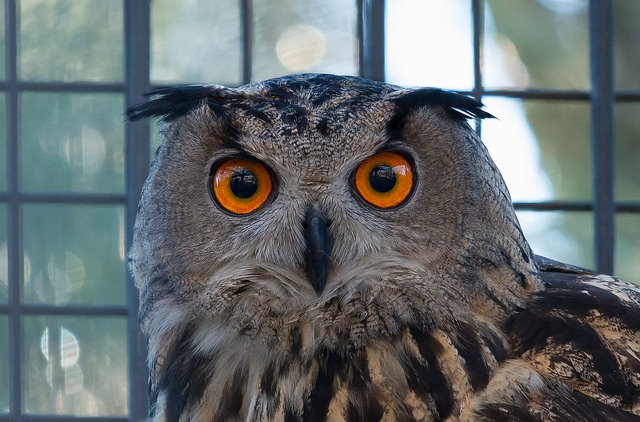
\includegraphics[width=4cm]{owl}
				\caption{Crazy Eyes - Eagle Owl by Orias1978 CC
				BY 2.0}
			\end{figure}

		\end{column}
		\begin{column}{0.48\textwidth}
			\begin{itemize}
				\item{Item 1}\footnotemark
				\item{Item 2}
				\item{Item 3}
			\end{itemize}
		\end{column}
	\end{columns}
	\footnotetext{dfjlsakjdf lsdkj flsdkjflsdakfjlsjflds
	flksdjfldkafjlsdkfj}
\end{frame}

\end{document}
